\documentclass[11pt,a4paper]{article}

% ---------- Packages ----------
\usepackage[utf8]{inputenc}
\usepackage[T1]{fontenc}
\usepackage{lmodern}
\usepackage{amsmath,amssymb,siunitx,booktabs}
\usepackage{enumitem}
\usepackage{geometry}
\usepackage{fancyhdr}
\usepackage[most]{tcolorbox}   % enhanced, breakable
\usepackage{hyperref}
\usepackage[siunitx]{circuitikz}

% ---------- Geometry ----------
\geometry{margin=2.5cm}

% ---------- Header/Footer ----------
\setlength{\headheight}{14pt}  % fancyhdr warning verhindern
\pagestyle{fancy}
\fancyhf{}
\lhead{Introduction to Electrical Engineering}
\cfoot{\thepage}

% ---------- Exercise Environment ----------
\newcounter{exercise}
\newenvironment{exercise}[1][]
  {\refstepcounter{exercise}%
   \begin{tcolorbox}[enhanced, breakable, width=\textwidth,
     colback=blue!5!white,colframe=blue!60!black,
     fonttitle=\bfseries\large,
     title=Exercise~\theexercise:~#1]}
  {\end{tcolorbox}}

% ---------- Solution Environment ----------
\newif\ifshowsolutions
\showsolutionstrue  % comment to hide solutions

\newenvironment{solution}
  {\ifshowsolutions
     \begin{tcolorbox}[enhanced, breakable, width=\textwidth,
       colback=green!5!white,colframe=green!50!black,
       fonttitle=\bfseries\large,
       title=Solution]}
  {\end{tcolorbox}\fi}

% ---------- Document ----------
\begin{document}

% ----- Header Box -----
\begin{tcolorbox}[enhanced, breakable, colback=gray!10!white,
  colframe=gray!70!black, fonttitle=\bfseries\large,
  title={Exercise Sheet \#7}, sharp corners, width=\textwidth]
\begin{center}
  AC 2
\end{center}
\end{tcolorbox}
\vspace{1cm}

% ----- Exercise 1 -----
\begin{exercise}[Equivalent Impedance]
Find $\underline{Z}_{eq}$ in the circuit below.

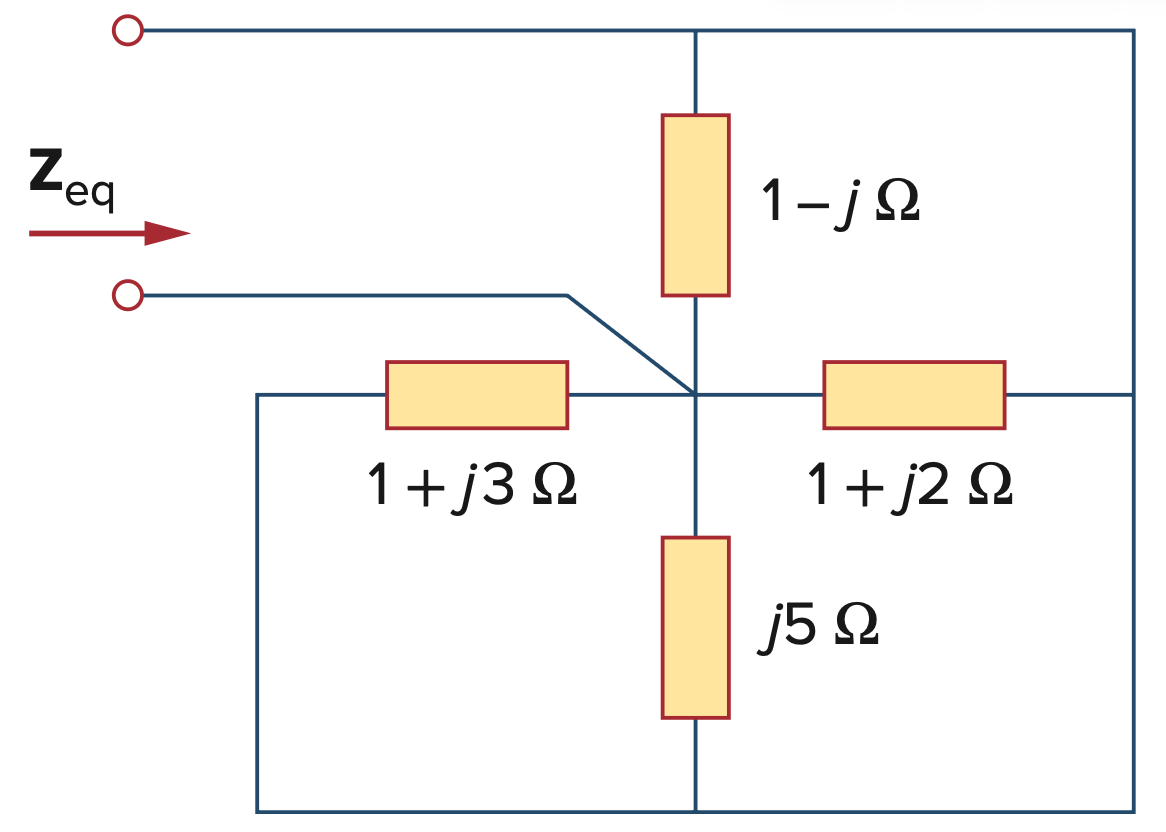
\includegraphics[width=0.7\textwidth]{figures/ACcircuit3.png}
\end{exercise}

\ifshowsolutions
\begin{solution}
\[
\underline{Y} = \frac{1}{\underline{Z}_1} + \frac{1}{\underline{Z}_2} + \frac{1}{\underline{Z}_3} + \frac{1}{\underline{Z}_4} = \frac{1}{1 - j} + \frac{1}{1 + j 2} + \frac{1}{1 + j 3} + \frac{1}{j 5}
\]
\[
= \frac{1 + j}{2} + \frac{1 - j 2}{5} + \frac{1 - j 3}{10} + \frac{-j 5}{25} = \frac{25 + 10 + 5 + j (25 - 20 - 15 - 10)}{50} = (0.8 - j 0.4)\,\text{S}
\]

\[
\underline{Z}_{eq} = \frac{1}{\underline{Y}} = \frac{1}{0.8 - j 0.4} = \frac{0.8 + j 0.4}{0.8^2 + 0.4^2} = (1 + j 0.5)\,\Omega
\]
\end{solution}
\fi

% ----- Exercise 2 -----
\begin{exercise}[Stepwise Voltage Division]
\begin{enumerate}[label=\alph*)]
  \item Calculate the phase shift of the circuit below.
  \item State whether the phase shift is leading or lagging (output with respect to input).
  \item Determine the magnitude of the output when the input is $120\,\text{V}$.
\end{enumerate}

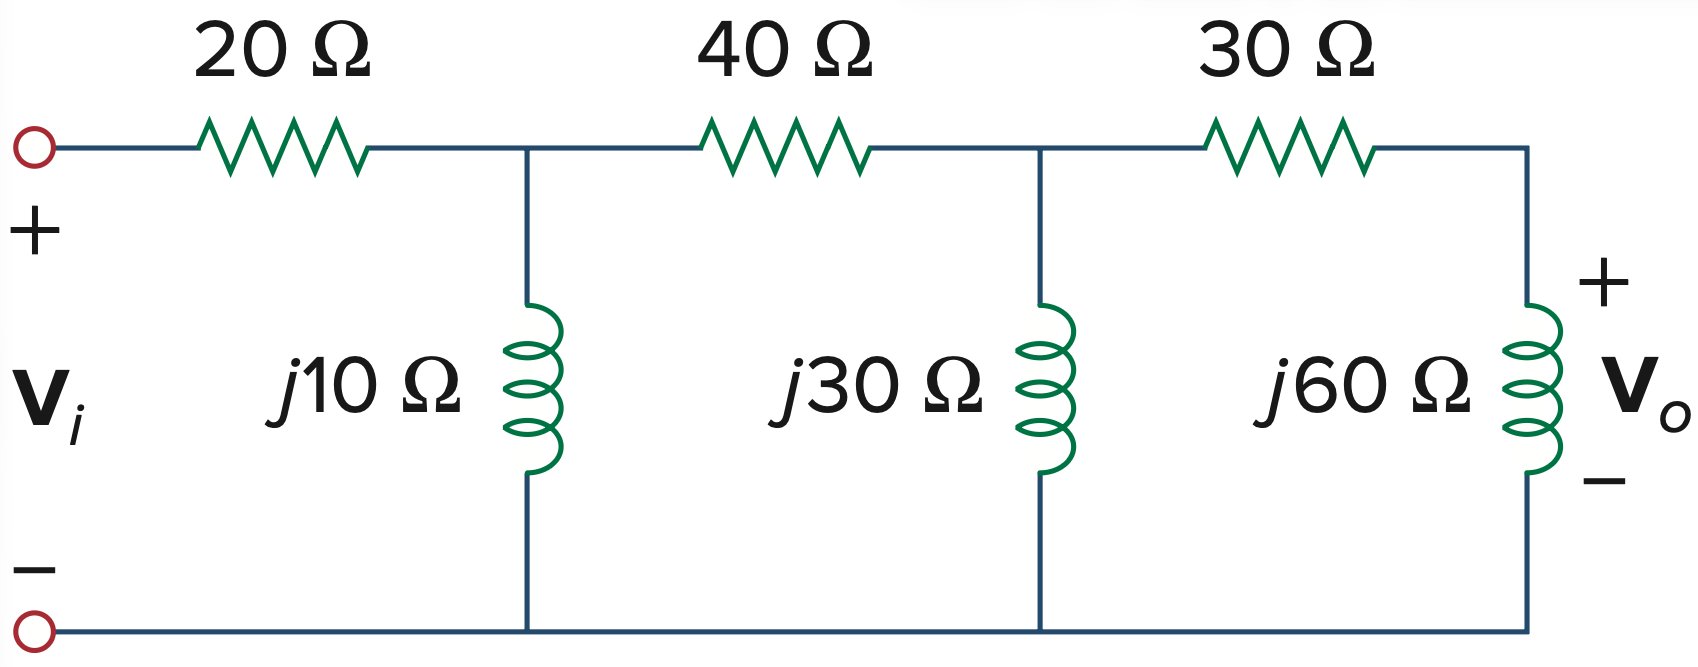
\includegraphics[width=0.7\textwidth]{figures/ACcircuit4.png}
\end{exercise}

\ifshowsolutions
\begin{solution}
\begin{enumerate}[label=\alph*)]
\item We take the input \(\underline{v}_i\) as the reference phasor (angle \(0^\circ\)) and denote the node voltages by \(\underline{v_1}, \underline{v}_2, \underline{v}_3\) (with \(\underline{v}_3 = \underline{v}_o\)).

Step 1: Relation between $\underline{v}_3$ and $\underline{v}_2$

Node 3 is a simple divider between the series resistor \(R_3\) and the inductor \(\underline{Z}_3\):
\[
\underline{v}_3 = \underline{v}_2 \cdot \frac{\underline{Z}_3}{R_3 + \underline{Z}_3}.
\]
With \(R_3 = 30,\; \underline{Z}_3 = j60\):
\[
\frac{\underline{v}_3}{\underline{v}_2} = \frac{j60}{30 + j60} = \frac{1}{1 - j 0.5} = 0.8 + 0.4\,j
\]
\[
= \sqrt{0.8^2 + 0.4^2} \cdot \exp\!\left(j \arctan\!\left(\frac{0.4}{0.8}\right)\right) = 0.894427 \cdot \exp(j 26.565^\circ).
\]

Step 2: Equivalent impedance seen from node 2

Node 2 sees \(\underline{Z}_2\) in parallel with the series path \(R_3 + \underline{Z}_3\):
\[
\underline{Z}_{\text{eq2}} = \frac{\underline{Z}_2 (R_3 + \underline{Z}_3)}{\underline{Z}_2 + (R_3 + \underline{Z}_3)}.
\]
With \(\underline{Z}_2 = j30\):
\[
R_3 + \underline{Z}_3 = 30 + j60,
\]
\[
\underline{Z}_{\text{eq2}} = \frac{j30 (30 + j60)}{j30 + (30 + j60)} = \frac{j900 - 1800}{30 + j90} = \frac{27000 + j189000}{9000} = 3 + j21.
\]

Now apply the divider between \(R_2\) and \(\underline{Z}_{\text{eq2}}\):
\[
\underline{v}_2 = \underline{v}_1 \cdot \frac{\underline{Z}_{\text{eq2}}}{R_2 + \underline{Z}_{\text{eq2}}}.
\]
\[
\frac{\underline{v}_2}{\underline{v}_1} = \frac{3 + j21}{40 + 3 + j21} = \frac{(3 + j21) (43 - j21)}{43^2 + 21^2} = \frac{57 + j84}{229}
\]
\[
= \frac{\sqrt{57^2 + 84^2}}{229} \cdot \exp\!\left(j \arctan\!\left(\frac{84}{57}\right)\right) = 0.443291 \cdot \exp\!\left(j 55.840^\circ\right).
\]

Step 3: Equivalent impedance seen from node 1

Node 1 sees \(\underline{Z}_1\) in parallel with the series path \(R_2 + \underline{Z}_{\text{eq2}}\):
\[
\underline{Z}_{\text{eq1}} = \frac{\underline{Z}_1 (R_2 + \underline{Z}_{\text{eq2}})}{\underline{Z}_1 + (R_2 + \underline{Z}_{\text{eq2}})}
\]

\[
R_2 + \underline{Z}_{\text{eq2}} = 40 + 3 + j21 = 43 + j21,
\]
\[
\underline{Z}_1 (R_2 + \underline{Z}_{\text{eq2}}) = j10 (43 + j21) = -210 + j430
\]
\[
\underline{Z}_1 + (R_2 + \underline{Z}_{\text{eq2}}) = j10 + (43 + j21) = 43 + j31
\]
Thus
\[
\underline{Z}_{\text{eq1}} = \frac{-210 + j430}{43 + j31} = \frac{(-210 + j430)(43 - j31)}{43^2 + 31^2} = \frac{4300 + j25000}{2810}
\]
\[
= \sqrt(4300^2 + 25000^2) \cdot \exp\!\left(j \arctan\!\left(25000/4300\right)\right) \cdot \frac{1}{2810} = 9.027439 \cdot \exp\!\left(j 80.241^\circ\right).
\]

Then the divider between \(R_1\) and \(\underline{Z}_{\text{eq1}}\) gives:
\[
\underline{v}_1 = \underline{v}_i \cdot \frac{\underline{Z}_{\text{eq1}}}{R_1 + \underline{Z}_{\text{eq1}}}.
\]
\[
R_1 + \underline{Z}_{\text{eq1}} = 20 + \frac{4300 + j25000}{2810} = \frac{20 \cdot 2810 + 4300 + j25000}{2810} = \frac{60500 + j25000}{2810}
\]
\[
= \sqrt(60500^2 + 25000^2) \cdot \exp\!\left(j \arctan\!\left(25000/60500\right)\right) \cdot \frac{1}{2810} = 23.296022 \cdot \exp\!\left(j 22.452^\circ\right)
\]
\[
\frac{\underline{v}_1}{\underline{v}_i} = \frac{9.027439}{23.296022} \cdot \exp\!\left(j (80.241^\circ - 22.452^\circ)\right) = 0.387510 \cdot \exp\!\left(j 57.789^\circ\right)
\]

Step 4: Combine the three ratios

Output relative to input:
\[
\frac{\underline{v}_o}{\underline{v}_i} = \frac{\underline{v}_3}{\underline{v}_i} = \frac{\underline{v}_3}{\underline{v}_2} \cdot\frac{\underline{v}_2}{\underline{v}_1} \cdot\frac{\underline{v}_1}{\underline{v}_i}
\]
\[
= 0.894427 \cdot \exp\!\left(j 26.565^\circ\right) \cdot 0.443291 \cdot \exp\!\left(j 55.840^\circ\right) \cdot 0.387510 \cdot \exp\!\left(j 57.789^\circ\right)
\]
\[
= 0.153644 \cdot \exp\!\left(j 140.194^\circ\right)
\]
\[
\Rightarrow \varphi = 140.2^\circ
\]

\item Since the phase shift is positive (\(+140.2^\circ\)), the output phasor **leads** the input phasor.

\item Magnitude of the output when \(V_i = 120\,\text{V}\):
\[
V_o = 0.153644 \cdot 120\,\text{V} \approx 18.44\,\text{V}
\]
\end{enumerate}
\end{solution}
\fi

% ----- Exercise 3 -----
\begin{exercise}[Nodal Analysis]
Determine $i$ in the circuit below.

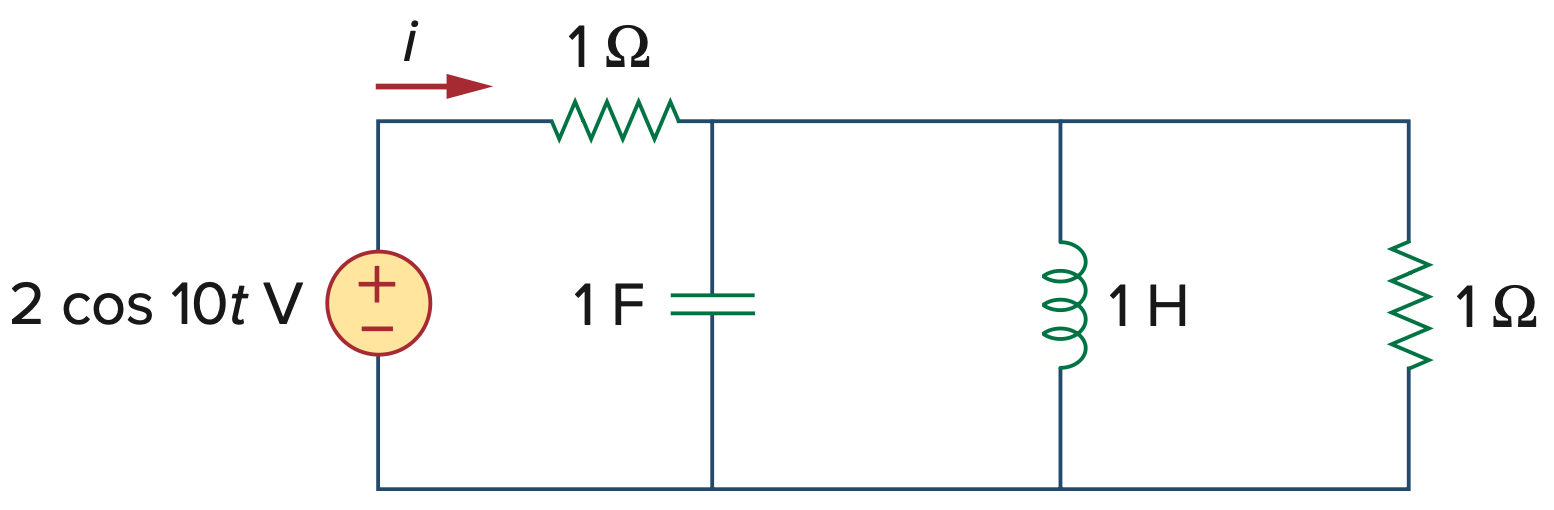
\includegraphics[width=0.7\textwidth]{figures/ACnodal.png}
\end{exercise}

\ifshowsolutions
\begin{solution}
\[
v_s(t) = 2\cos(10t)\quad\Rightarrow\quad \omega=10
\]
Capacitor and inductor admittances (1\,F and 1\,H):
\[
\underline{Y}_C = j\omega C = j10,\qquad \underline{Y}_L = \frac{1}{j\omega L} = -\frac{j}{10} = -j0.1,
\]
and the parallel resistor gives \(R = 1\). Thus the total admittance of the parallel block is
\[
\underline{Y} = R + \underline{Y}_C + \underline{Y}_L = 1 + j10 - j0.1 = 1 + j9.9.
\]

KCL at the node (current through series \(1\Omega\) equals current into the parallel block):
\[
\frac{\hat{v}_s - \underline{\hat{v}}}{1} = \underline{\hat{v}}\;\underline{Y}
\quad\Longrightarrow\quad
\underline{\hat{v}}\,(1 + \underline{Y}) = \hat{v}_s
\quad\Longrightarrow\quad
\underline{\hat{v}} = \frac{\hat{v}_s}{1 + \underline{Y}}.
\]
The source current \( \underline{\hat{i}}\) (which is \(i\) in time domain) is the current through the series \(1\Omega\):
\[
\underline{\hat{i}} = \frac{\hat{v}_s - \underline{\hat{v}}}{1} = \hat{v}_s \frac{\underline{Y}}{1 + \underline{Y}}
\]

Substitute \(\underline{Y} = 1 + j9.9\):
\[
\underline{\hat{i}} = 2 \cdot \frac{1 + j9.9}{2 + j9.9} = \frac{200.02 + j19.8}{102.01} \approx (1.9608 + j0.1941)\,\text{A}
\]

Magnitude, phase and back to the time domain (cosine reference):
\[
i(t) = 1.9704\cos\big(10t + 5.655^\circ\big)\,\text{A}
\]
\end{solution}
\fi

% ----- Exercise 4 -----
\begin{exercise}[Instantaneous and Average Power]
If $v(t)=160\cos(50t)\,\text{V}$ and $i(t)=-33\sin(50t-30^\circ)\,\text{A}$, calculate the instantaneous power and the average power.
\end{exercise}

\ifshowsolutions
\begin{solution}
First rewrite the current using
\[
\sin x = \cos(x-90^\circ):
\]
\[
i(t)=-33\cos\!\big[(50t-30^\circ)-90^\circ\big] = -33\cos(50t-120^\circ).
\]

The instantaneous power is
\[
p(t) = v(t)i(t) =160\cos(50t)\,\big[-33\cos(50t-120^\circ)\big] = -5280\cos(50t)\cos(50t-120^\circ).
\]

Use the identity
\[
\cos A \cos B = \tfrac12\left[\cos(A-B)+\cos(A+B)\right].
\]

Let \(A = 50t\), \(B = 50t-120^\circ\):
\[
p(t) = -5280 \cdot \tfrac12\left[\cos\big(120^\circ\big)+\cos\big(100t-120^\circ\big)\right] = -2640\left[\cos 120^\circ + \cos(100t-120^\circ)\right].
\]

Since \(\cos 120^\circ = -\tfrac12\),
\[
p(t) = -2640\left[-\tfrac12 + \cos(100t -120^\circ)\right] = 1320 - 2640\cos(100t-120^\circ).
\]

Thus the **instantaneous power** is
\[
\boxed{p(t)=1320 + 2640\cos(100t+60^\circ)\ \text{W}}.
\]

The **average power** is the DC term:
\[
\boxed{\overline{P} = 1320\ \text{W}}.
\]
\end{solution}
\fi

% ----- Exercise 5 -----
\begin{exercise}[Complex Power Calculation]
For the entire circuit below, calculate:
\begin{enumerate}[label=\alph*)]
  \item the complex power
  \item the average power delivered by the source
  \item the reactive power
  \item the apparent power
  \item the power factor
\end{enumerate}

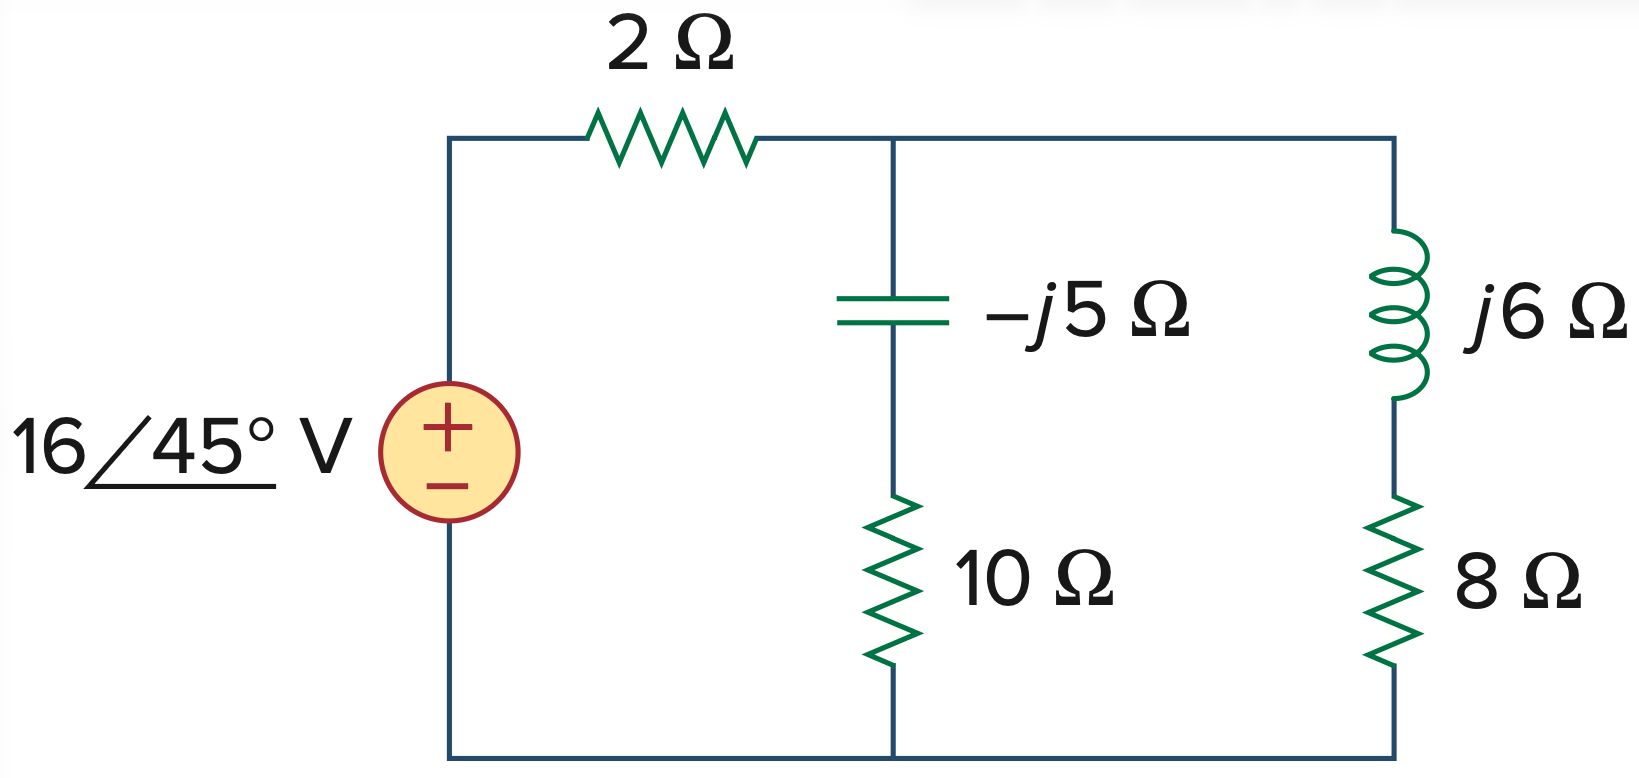
\includegraphics[width=0.7\textwidth]{figures/complex_power.png}
\end{exercise}

\ifshowsolutions
\begin{solution}
Two parallel branches after the 2\(\Omega\) resistor:
\[
\underline{Z}_1 = 10 - j5,\qquad \underline{Z}_2 = 8 + j6.
\]

Total impedance (including the 2\(\Omega\) resistor in series):
\[
\underline{Z} = 2 + \left(\frac{1}{\underline{Z}_1} + \frac{1}{\underline{Z}_2}\right)^{-1} = 2 + \Big(\frac{1}{10-j5} + \frac{1}{8+j6}\Big)^{-1}
\]
\[
= 2 + \Big(\frac{10+j5}{100+25} + \frac{8-j6}{64+36}\Big)^{-1} = 2 + \Big(0.08 + j0.04 + 0.08 - j\,0.06\Big)^{-1}
\]
\[
= 2 + \frac{0.16 + j\,0.02}{0.16^2 + 0.02^2} = 2 + \frac{0.16 + j\,0.02}{0.026} = \frac{0.212 + j\,0.02}{0.026}\,\Omega
\]
\[
Z = \frac{\sqrt(0.212^2 + 0.02^2)}{0.026} \approx 8.1901\,\Omega
\]
\[
\varphi = \arctan\!\frac{0.02}{0.212} = 5.39^\circ
\]

Source voltage (phasor complex RMS value):
\[
\underline{V}_s = 16 \cdot e^{j\,45^\circ} = (11.3137 + j\,11.3137)\,\text{V}
\]
Source current (phasor complex RMS value):
\[
\underline{I}_s = \frac{\underline{V}_s}{\underline{Z}} = \frac{16}{8.1901} \cdot e^{j\,(45^\circ - 5.39^\circ)} = 1.9536 \cdot e^{j\,39.61^\circ} = (1.5051 + j\,1.2455)\,\text{A}
\]

\begin{enumerate}[label=\alph*)]
\item Complex power delivered by the source:
\[
\underline{S} = \underline{V}_s \underline{I}_s^* = (11.3137 + j\,11.3137)\,\text{V} \cdot (1.5051 - j\,1.2455)\,\text{A} = (31.12 + j\,2.94)\,\text{VA}.
\]

\item Active power delivered by source:
\[
P = \text{Re}(\underline{S}) = 31.12\,\text{W}
\]

\item Reactive power:
\[
Q = \text{Im}(\underline{S}) = 2.94\,\text{VAR}
\]

\item Apparent power:
\[
S = \sqrt{P^2 + Q^2} = 31.26\,\text{VA}.
\]

\item Power factor (scalar) and type:
\[
\cos \varphi = \dfrac{P}{S} = \dfrac{31.12}{31.26} \approx 0.9956.
\]
Since \(Q>0\) the net load is inductive, so the power factor is \emph{lagging}.
\end{enumerate}
\end{solution}
\fi

% ----- Exercise 6 -----
\begin{exercise}[RMS Values and Average Power]
The voltage across a load and the current through it are given by
$v(t)=20+60\cos(100t)\,\text{V}$ and $i(t)=1-0.5\sin(100t)\,\text{A}$.
Find:
\begin{enumerate}[label=\alph*)]
  \item the RMS values of the voltage and of the current
  \item the average power dissipated in the load
\end{enumerate}
\end{exercise}

\ifshowsolutions
\begin{solution}
\begin{enumerate}[label=\alph*)]
\item For a signal composed of a constant (DC) term plus a single sinusoid,
\[
x(t) = X_{\mathrm{DC}} + \hat{x} \cos(\omega t+\phi),
\]
the mean square (time average of \(x^2(t)\)) over one period is
\[
\overline{x^2(t)} = X_{\mathrm{DC}}^2 + \frac{\hat{x}^2}{2},
\]
because the cross term between DC and the sinusoid averages to zero and the sinusoid contributes \(\hat{x}^2/2\). Thus the RMS value is
\[
X = \sqrt{X_{\mathrm{DC}}^2 + \dfrac{\hat{x}^2}{2}}.
\]

Apply this to the voltage:
\[
V_{\mathrm{DC}} = 20,\qquad \hat{v} = 60
\]
Hence
\[
V = \sqrt{20^2 + \frac{60^2}{2}} = \sqrt{2200} = 10\sqrt{22} \approx 46.9\,\text{V}.
\]

Apply the same formula to the current. Write the current as
\[
i(t) = I_{\mathrm{DC}} + \hat{i} \cos(100t + \phi_i).
\]
Here \(I_{\mathrm{DC}} = 1\). The AC term is \(-0.5 \sin(100t)\), which has amplitude \(\hat{i} = 0.5\). (The sign and phase do not affect the RMS magnitude.) Thus
\[
I = \sqrt{1^2 + \frac{(0.5)^2}{2}} = \sqrt{1.125} \approx 1.061\,\text{A}.
\]

\item The instantaneous power is
\[
p(t) = v(t) i(t) = (20 + 60 \cos(100t))\bigl(1 - 0.5 \sin(100t)\bigr).
\]
Expand:
\[
p(t) = 20 \cdot 1 + 20 \cdot (-0.5 \sin(100t)) + 60 \cos(100t) \cdot 1 + 60 \cos(100t) \cdot (-0.5 \sin(100t))
\]
\[
= 20 - 10 \sin(100t) + 60 \cos(100t) - 30 \cos(100t) \sin(100t)
\]
The average power \(P\) is the time average of \(p(t)\) over one period. Every pure sinusoid (or product of sinusoids of the same frequency that reduces to a sinusoid at twice the frequency) has zero average. Thus the time average of \(-10 \sin(100t)\), of \(60 \cos(100t)\), and of \(-30 \cos(100t) \sin(100t)\) is zero. Therefore only the DC term remains:
\[
P = \overline{p(t)} = 20\,\text{W}
\]

Alternatively, using the decomposition into DC and sinusoidal parts:
\[
P = V_{\mathrm{DC}}I_{\mathrm{DC}} + \frac{1}{2} \hat{v} \hat{i} \cos\varphi,
\]
where \(\varphi\) is the phase difference between the voltage and current sinusoids. Here \(V_{\mathrm{DC}} I_{\mathrm{DC}} = 20 \cdot 1\) and the sinusoidal part has
\[
\hat{v} = 60,\qquad \hat{i} = 0.5.
\]
Voltage sinusoid: \(60 \cos(100t)\) (phase \(0\)). Current sinusoid: \(-0.5 \sin(100t) = 0.5 \cos(100t + \tfrac{\pi}{2})\) (phase \(+\tfrac{\pi}{2}\)). Thus \(\varphi = 0 - (+\tfrac{\pi}{2}) = -\tfrac{\pi}{2}\) and \(\cos\varphi = \cos(-\tfrac{\pi}{2}) = 0\). Hence the sinusoidal contribution is zero and
\[
P = 20\,\text{W}.
\]
\end{enumerate}
\end{solution}
\fi

% ----- Exercise 7 -----
\begin{exercise}[Complex Network Analysis]
Given the following network with a sinusoidal voltage source $U = 230\,\mathrm{V}$, $f = 50\,\mathrm{Hz}$ and the components $R = 20\,\Omega$, $L = 100\,\mathrm{mH}$:

\begin{center}
\begin{circuitikz}[european, scale=1]
  \draw
  (0,0) to[V, l_=$U$] (0,3)
        to[R=$R$] (3,3)
        to[L=$L$] (6,3)
        -- (6,0) -- (0,0);
\end{circuitikz}
\end{center}

Determine:

\begin{enumerate}
  \item the complex impedance $Z$,
  \item the RMS current $I$,
  \item the phase shift between current and voltage,
  \item the power factor $\cos\varphi$,
  \item the active power $P$,
  \item the reactive power $Q$.
\end{enumerate}
\end{exercise}

\ifshowsolutions
\begin{solution}
\[
\omega = 2\pi f = 314\,\text{rad/s}
\]
\[
X_L = \omega L = 31.4\,\Omega
\]
\[
\underline{Z} = (20 + j31.4)\,\Omega \Rightarrow |\underline{Z}| = 37.2\,\Omega
\]
\[
I = \frac{230}{37.2} = 6.18\,\text{A}
\]
\[
\varphi = \arctan\left(\frac{31.4}{20}\right) = 57.5^\circ
\]
\[
\cos\varphi = 0.54
\]
\[
P = U I \cos\varphi = 764\,\text{W}
\]
\[
Q = U I \sin\varphi = 1199\,\text{VAR}
\]
\end{solution}
\fi

% ----- Exercise 8 -----
\begin{exercise}[Reactive Power Compensation]
An AC motor with impedance $\underline{Z} = 4.2 + j\,3.6\,\Omega$ is supplied by a 220-V, 60-Hz source.
\begin{enumerate}[label=\alph*)]
  \item Find the power factor, the real power P, and the reactive power Q.
  \item Determine the capacitor required to be connected in parallel with the motor so that the power factor is corrected to unity.
\end{enumerate}
\end{exercise}

\ifshowsolutions
\begin{solution}
\begin{enumerate}[label=\alph*)]
\item The magnitude and angle of the load impedance are
\[
|\underline{Z}| = \sqrt{R^2 + X^2} = \sqrt{4.2^2 + 3.6^2} \approx 5.532\,\Omega,
\]
\[
\varphi = \arctan\!\frac{X}{R} = \arctan\!\frac{3.6}{4.2} \approx 0.709\,\text{rad} \approx 40.6^\circ.
\]

The RMS current is
\[
I = \frac{V}{|\underline{Z}|} = \frac{220}{5.532} \approx 39.77\,\mathrm{A}.
\]

The power factor (PF) is the cosine of the impedance angle (lagging because \(X>0\)):
\[
\cos \varphi \approx 0.76\quad\text{(lagging)}.
\]

Compute the complex power:
\[
\underline{S} = \underline{V} \underline{I}^* = \underline{V} \frac{\underline{V}^*}{\underline{Z}^*} = \frac{V^2}{\underline{Z}^*} = V^2/(R - jX)^* = \frac{V^2(R + jX)}{R^2 + X^2}
\]

So the real and reactive powers are
\[
P = \frac{V^2 R}{R^2 + X^2} \approx 6.643\,\mathrm{kW},
\]
\[
Q = \frac{V^2 X}{R^2 + X^2} \approx 5.694\,\mathrm{kVAR}.
\]

\item To correct the power factor to unity we must supply capacitive reactive power \(Q_C\) that cancels the motor's inductive reactive power \(Q\). For a capacitor connected in parallel across the same RMS voltage \(V\),
\[
|Q_C| = V^2 \,\omega C,\qquad \omega = 2\pi f.
\]

We need \( |Q_C| = Q \), hence
\[
C = \frac{Q}{V^2 \omega} = \frac{5694}{220^2 \cdot 2\pi \cdot 60} \approx 312\,\mu\mathrm{F}.
\]
\end{enumerate}
\end{solution}
\fi

% ----- Exercise 9 -----
\begin{exercise}[Series Resonance]
A series $RLC$ network has $R = 2\,\text{k}\Omega$, $L = 40\,\text{mH}$, and $C = 1\,\mu\text{F}$. Calculate the impedance at resonance and at one-fourth, one-half, twice, and four times the resonant frequency.
\end{exercise}

\ifshowsolutions
\begin{solution}
For s series RLC network with
\[
R=\SI{2}{\kilo\ohm},\qquad L=\SI{40}{\milli\henry},\qquad C=\SI{1}{\micro\farad}
\]
the series impedance is
\[
\underline{Z}(j\omega)=R+j\bigl(\omega L-\tfrac{1}{\omega C}\bigr).
\]

Resonance occurs when the net reactance is zero:
\[
\omega_0=\frac{1}{\sqrt{LC}}
\]
Substitute the values:
\[
\omega_0=\frac{1}{\sqrt{(40\times10^{-3})(1\times10^{-6})}}=\SI{5000}{\radian\per\second}
\]

For a given angular frequency \(\omega\),
\[
X_L=\omega L,\qquad X_C=\frac{1}{\omega C},\qquad X=X_L-X_C,
\]
\[
\underline{Z} = R + jX,\qquad |\underline{Z}| = \sqrt{R^2 + X^2},\qquad \varphi = \arctan\!\frac{X}{R}.
\]

We evaluate at \(\omega = k\omega_0\) for \(k=\tfrac14,\tfrac12,1,2,4\).

\bigskip
\begin{tabular}{@{}lcccccc@{}}
\toprule
$k$ & $\omega$ (rad/s) & $X_L$ (\si{\ohm}) & $X_C$ (\si{\ohm}) & $\underline{Z}$ (\si{k\ohm}) & $|\underline{Z}|$ (\si{k\ohm}) & $\varphi$ \\
\midrule
$0.25$ & $1250$ & $50$ & $800$ & $2 - j0.75$ & $2.136$ & $-20.6^\circ$ \\[4pt]
$0.5$ & $2500$ & $100$ & $400$ & $2 - j0.3$ & $2.022$ & $-8.5^\circ$ \\[4pt]
$1$ & $5000$ & $200$ & $200$ & $2$ & $2$ & $0^\circ$ \\[4pt]
$2$ & $10000$ & $400$ & $100$ & $2 + j0.3$ & $2.022$ & $+8.5^\circ$ \\[4pt]
$4$ & $20000$ & $800$ & $50$ & $2 + j0.75$ & $2.136$ & $+20.6^\circ$ \\
\bottomrule
\end{tabular}

\bigskip
\noindent Observations:
\begin{itemize}
  \item At resonance ($k=1$) the inductive and capacitive reactances cancel, leaving purely resistive impedance \(Z=R=\SI{2000}{\ohm}\).
  \item The network is capacitive ($X<0$) for frequencies below resonance and inductive ($X>0$) for frequencies above resonance.
  \item The magnitudes at pairs \(k=\tfrac14\) and \(k=4\) are equal (symmetry), and likewise for \(k=\tfrac12\) and \(k=2\).
\end{itemize}
\end{solution}
\fi

% ----- Exercise 10 -----
\begin{exercise}[Parallel Resonance]
Rework Exercise 6 if the elements are connected in parallel.
\end{exercise}

\ifshowsolutions
\begin{solution}
For the parallel connection the total admittance is
\[
\underline{Y}(j\omega) = \underbrace{\frac{1}{R}}_{G} + j\Bigl(\underbrace{\omega C}_{B_C} + \underbrace{\Bigl(-\frac{1}{\omega L}\Bigr)}_{B_L}\Bigr) = G + jB(\omega).
\]
The impedance is the reciprocal of the admittance:
\[
\underline{Z}(\omega) = \frac{1}{\underline{Y}(\omega)} = \frac{1}{G+jB} = \frac{G-jB}{G^2+B^2}
\]
Its magnitude and phase are
\[
|\underline{Z}|=\frac{1}{\sqrt{G^2+B^2}},\qquad \varphi = \operatorname{atan2}\bigl(\text{Im}(\underline{Z}),\text{Re}(\underline{Z})\bigr) = \arctan\!\frac{-B}{G}.
\]

Parallel resonance (net susceptance zero) occurs at the same angular frequency as series resonance:
\[
B(\omega_0) = 0 \quad\Rightarrow\quad \omega_0 = \frac{1}{\sqrt{LC}}
\]
With the given values
\[
\omega_0 = \frac{1}{\sqrt{(40\times10^{-3})(1\times10^{-6})}} = \SI{5000}{\radian\per\second}.
\]
Also
\[
G = \frac{1}{R} = \frac{1}{2000} = \SI{5e-4}{\siemens}.
\]

At resonance $B(\omega_0)=0$, so
\[
Y(\omega_0) = G \qquad\Rightarrow\qquad Z(\omega_0) = \frac{1}{G} = R = \SI{2000}{\ohm}.
\]

We compute for each ratio \(k\):
\[
\omega = k\omega_0,\qquad B = \omega C-\frac{1}{\omega L},\qquad \underline{Z} = \frac{G-jB}{G^2+B^2}
\]

\bigskip
\begin{tabular}{@{}lcccccc@{}}
\toprule
$k$ & $\omega$ (rad/s) & $B_C$ (\si{m\ohm}) & $B_L$ (\si{m\ohm}) & $\underline{Z}$ (\si{\ohm}) & $|\underline{Z}|$ (\si{\ohm}) & $\varphi$ \\
\midrule
$0.25$ & $1250$ & $1.25$ & $20$ & $1.42 + j\,53.30$ & $53$ & $+88.5^\circ$ \\[4pt]
$0.5$ & $2500$ & $2.5$ & $10$ & $8.85 + j\,132.74$ & $133$ & $+86.2^\circ$ \\[4pt]
$1$ & $5000$ & $5$ & $5$ & $2000$ & $2000$ & $0^\circ$ \\[4pt]
$2$ & $10000$ & $10$ & $2.5$ & $8.85 - j\,132.74$ & $133$ & $-86.2^\circ$ \\[4pt]
$4$ & $20000$ & $20$ & $1.25$ & $1.42 - j\,53.30$ & $53$ & $-88.5^\circ$ \\
\bottomrule
\end{tabular}

\bigskip
\noindent Notes on the results:
\begin{itemize}
  \item At resonance the susceptances of the inductor and capacitor cancel and the parallel branch behaves as a pure conductance $G$, giving $Z(\omega_0)=R$.
  \item For frequencies below resonance ($k<1$) the net susceptance $B$ is negative (inductive behavior), producing an impedance with a large positive imaginary part (inductive reactance).
  \item For frequencies above resonance ($k>1$) $B$ is positive (capacitive behavior), producing impedance with a large negative imaginary part (capacitive reactance).
  \item The impedances occur in conjugate pairs for reciprocal frequency ratios (e.g. $k=0.25$ and $k=4$; $k=0.5$ and $k=2$).
\end{itemize}
\end{solution}
\fi

\end{document}